\lipsum[1]

\subsection{Subsection 1}
\label{sec:subsection_res_1}

\lipsum[2]

\subsubsection{Subsubsection 1.1}
\label{sec:subsubsec_res_1.1}

\lipsum[3]

\subsubsection{Subsubsection 1.2}
\label{sec:subsubsec_res_1.2}

\lipsum[4]

% example of a plot with referring to it

Based on the possible structure of the product and on other obtained information, a probable reduction mechanism can be drawn (Fig.~\ref{fig:IR_OPAmech}). 

\begin{figure}[!ht]
  \centering
 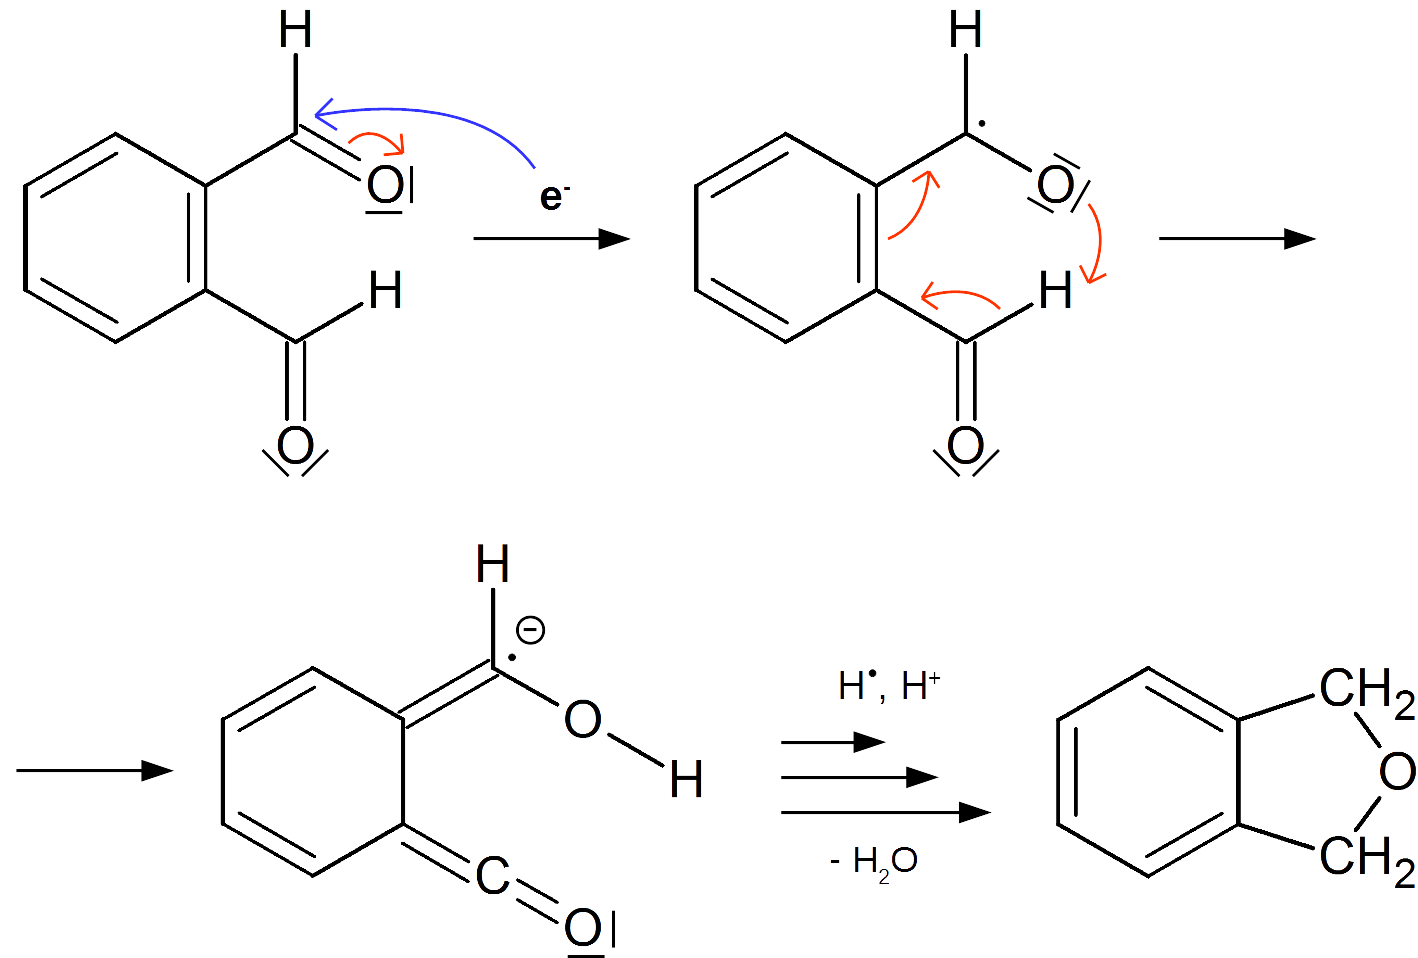
\includegraphics[width=11cm]{IR_OPAmech.png}
 \caption{A proposed mechanism for the first step of the OPA reduction.}
 \label{fig:IR_OPAmech}
\end{figure}

% following is an example of a broader plot on an individual landscape page

\begin{landscape}
\begin{figure}[!ht]
  \centering
 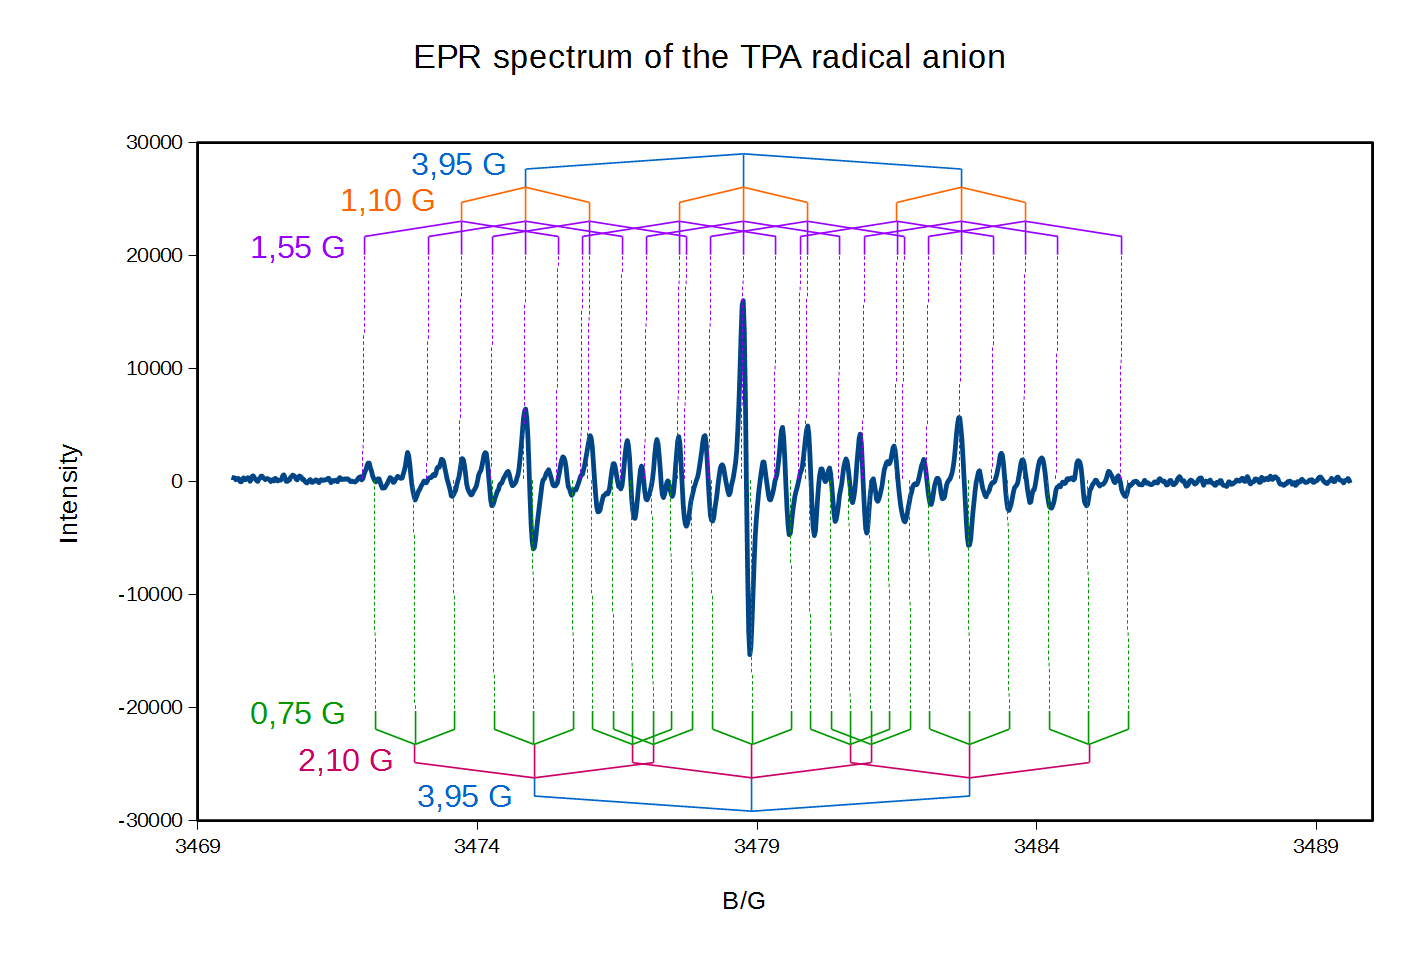
\includegraphics[width=18cm]{EPR_TPA.png}
 \caption[EPR spectrum of the TPA radical anion.]{EPR spectrum of the TPA radical anion generated electrochemically \textit{in~situ} in the EPR cavity. Derived coupling constants for the \textit{cis} and \textit{trans} rotamer are displayed above and below the spectrum.}
 \label{fig:EPR_TPA}
\end{figure}

\end{landscape}

% example of a table with a reference

Table~\ref{tab:tableXPABA} summarizes reduction potentials and the electron consumptions in both steps. For comparison of the reduction behavior, the value of reduction potential of benzaldehyde is given.

\begin{table}[htb]
\centering
\caption{Reduction potentials and the electron consumptions for studied benzenedialdehydes in ACN and comparison with benzaldehyde (BA).}
\begin{tabular}{ c c c c c c }
\toprule
& $E_{red}^1$/V & $z_1$ & $E_{red}^2$/V & $z_2$ & $E_{red}^3$/V  \\ 
\midrule
    OPA & $-1.51$ & 0.40 & $-2.02$ & 1 & ($-2.20$) \\ 
	IPA & $-1.68$ & 0.80 & $-2.04$ & $>$ 1 & -- \\ 
	TPA & $-1.46$ & 0.35 & $-1.90$ & $<$ 1 & -- \\ 
	BA\cite{Mairanovskii1976} & \ & \  & $-2.00$  & \ &  \\ 
\bottomrule
\end{tabular}
\label{tab:tableXPABA}
\end{table}

% example of a more complex table with a multicolumn

\begin{table}[!ht]
  \begin{center}
	\caption{Reduction potentials from CV for OPA in ACN, DMF and acetone and on mercury and gold electrode. Potentials are related to the SCE.}
  \label{tab:OPAnevoda}
  \footnotesize
	\renewcommand{\arraystretch}{1.4}
\begin{tabular}{ >{\centering\arraybackslash} m{1.7cm}  c  c  c  c  c  c  c  }
\toprule
	\shortstack{solvent/\\electrode} & E$_{pc}^1$/V & E$_{pa}^1$/V & $\Delta$E$^1$/mV & E$_{pc}^2$/V & E$_{pa}^2$/V & $\Delta$E$^2$/mV & E$_{pc}^3$/V \\  
\midrule[0.3mm]	
	  ACN/Hg & $-1.51$  & $-1.45$ & 60 & $-2.02$ & -- & -- & $-2.20$   \\ 
	  DMF/Hg & $-1.41$ & $-1.35$ & 60 & $-2.10$ & $-2.02$ & 80 & --   \\ 
	  DMF/Au & $-1.44$ & $-1.37$ & 70 & -- & -- & -- & --   \\ 
	  acetone/Hg & \multicolumn{7}{c}{the substance probably reacts with the solvent} \\ 
\bottomrule	   
\end{tabular}
\end{center}
\end{table}

% another table example

\begin{table}[!ht]
  \begin{center}
	\caption{Slopes from \emph{ln(i)-t} curves for the ratio AA:OPA 3:1}
  \label{tab:slopesAAs}
	\renewcommand{\arraystretch}{1.4}
\begin{tabular}{l >{\centering\arraybackslash}m{2.5cm} >{\centering\arraybackslash}m{2.5cm}}
\toprule
\multicolumn{1}{c}{AA:OPA 3:1}  & \multicolumn{2}{c}{slope: $\frac{dln(i)}{dt}\cdot10^3$} \\ 
 \toprule
\multicolumn{1}{c}{amino acid}  & pH 7.86    & pH 11.22 \\ 
\midrule[0.3mm]
   glycine                         & -3.20   & -3.65  \\
   alanine                         & -2.00   & -5.10 \\ 
	 $\alpha$-aminobutyric acid      & -1.70   & -4.70 \\
	 $\alpha$-aminoisobutyric acid   & -0.04   & -0.20 \\
	 valine                          & -1.40   & -2.70 \\
	 norvaline                       & -1.70   & -4.25 \\
	 leucine                         & -1.75   & -3.80 \\
	 isoleucine                      & -1.40   & -2.90 \\
\bottomrule
\end{tabular}
\end{center}
\end{table}
